\section{Conclusion}
\begin{frame}{Conclusion}
\begin{itemize}
    \item Graph learning beyond DAGs, TFs, and small graphs
% Many methods and models have been proposed and examined for graph inference, but each have details separating them from the work discussed here. Many either rely on DAGs, or model direct interactions, which often completely ignores protein kinases and instead only focuses on transcription factors. The justification is often that transcription factors are complicated enough on their own, which can be interpreted from the results in section~\autoref{sec:yeast_results}. It is found that the method clearly outperform LLC on the indirect edges from PKs. It is found that the indirect evidence of protein interaction gathered from knockout studies are not convincingly useful by itself for inference, but does seem to add useful information.

% We demonstrate, that it is possible to simulate non-linear and complex gene regulation involving protein kinases, and infer the underlying interactions, in spite of the much larger space of parameters defining the simulations~(\autoref{sec:dream_results}). It is also demonstrated that performance can be improved significantly with a novel loss function~(\autoref{sec:cascade_loss}).
    \item Future work
    \begin{itemize}
        \item PK$\rightarrow$TF vs PK$\rightarrow$PK preference
        \begin{itemize}
            \item Outgoing edges usually sum to <1 for mediating PK
% When an effect from a protein kinase knockout is observed across a node value, the equilibrium method can choose to infer an edge to the most obvious transcription factor or infer an edge to another protein kinase that are found to regulate the same transcription factors~(\autoref{sec:toy}).
% If we use L1-regularization for PK edges the latter is only favored in the case where the weights from the other PK sum to more than 1.
% Testing the performance improvements possible with the alternative loss function described in~\autoref{sec:cascade_loss} would be interesting for simulated data on larger networks. It could be a great way to improve performance on simulated data, however, it is unclear how much this would help for experimental data.
        \end{itemize}
    \item Exploiting other data types
% As discussed in~\autoref{sec:evolution} there are potential in interspecies data, which can be exploited in order to take advantage of data from similar species, instead of studying a strain in isolation. This can especially be useful if one were to study an organism which is not a major model organism as has been done here. It can be implemented into the current model by defining a new loss function inspired by the one applied by Kashima~et~al.~\cite{Kashima2009}. Their method was however inferring undirected edges for enzyme interactions, which can be a problem to consider if we are interested in directed edges.
        \begin{itemize}
            \item Evolutionary cost
            \item Interspecies protein similarity 
            % ($\text{W}^{(k,l)}, k \ne l$)
            \item Intraspecies gene expression similarity 
            % ($\text{W}^{(k,l)}, k = l$)
            \item Multiple observations of same KO
        \end{itemize}
    \item Further extension to GeneNetWeaver
% It could be interesting to increase model realism, for instance by considering cell compartmentalization, cell cycle, time-dependence of processes, allowing proteins more than two phosphorylation states etc.
% Currently, the GeneNetWeaver kinase extension was written to use kinases as the signal transducing proteins and phosphatases collectively included in the model by the constant decay of phosphates on phosphorylated proteins~(\autoref{sec:gnw_extension}). Although, allowing negative protein kinase edges, corresponding to targeted dephosphorylation, was tested to work without issue~(\autoref{fig:micro_average.d}).
% Transcription factors can both have an active form as phosphorylated and as unphosphorylated. Allowing the unphosphorylated transcription factor to serve an active regulation role could be a further extension to increase realism of simulation.
    \begin{itemize}
        \item Phosphorylation $\ne$ activity
        \item Nondimensionalization
    \end{itemize}
\end{itemize}
\end{itemize}
\end{frame}

\begin{frame}{Nondimensionalized kinase regulation model}
\begin{columns}
\begin{column}{0.7\textwidth}
Kinase cascade, each protein with single input
\begin{subequations}
\begin{align}
\dv{\phi_i}{t} &=
    w_i \phi_{i-1} \left(p_i - \phi_i\right) - \lambda_i^{(\text{Phos})} \phi_i    
\\
    &=
    \frac{\hat{w}_i}{p_{i-1}^{(\text{max})}} \hat{\phi}_{i-1} p_{i-1}^{(\text{max})} \left(\hat{p}_i p_i^{(\text{max})} - \hat{\phi}_i p_i^{(\text{max})} \right) - \lambda_i^{(\text{Phos})} \hat{\phi}_i p_i^{(\text{max})}
\\
\phi_i &= \hat{\phi}_i p_i^{(\text{max})} \implies
\\
\dv{\hat{\phi}_i}{t} &=
    \hat{w}_i \hat{\phi}_i \left(\hat{p}_i - \hat{\phi}_i\right) - \lambda_i^{(\text{Phos})} \hat{\phi}_i
\end{align}
\end{subequations}
Generalized, any protein can affect any protein
\begin{subequations}
\begin{align}
\dv{\hat{\phi}_i}{t} &=
    \left( \sum_j \hat{w}_{ij} \hat{\phi}_j \right) \left(\hat{p}_i - \hat{\phi}_i\right) - \lambda_i^{(\text{Phos})} \hat{\phi}_i
\\
\dv{\hat{\boldsymbol{\phi}}}{t} &= 
    \left(\hat{W} \hat{\boldsymbol{\phi}}\right) \left(\hat{\boldsymbol{p}} - \hat{\boldsymbol{\phi}}\right) - \Lambda_\text{Phos} \hat{\boldsymbol{\phi}}
\end{align}
\end{subequations}
Before: $\dv{\boldsymbol{\phi}}{t} = (W \boldsymbol{\phi}) \left(1 - \frac{\boldsymbol{\phi}}{\boldsymbol{p}}\right) - \Lambda_\text{Phos} \boldsymbol{\phi}$
\end{column}

\begin{column}{0.3\textwidth}
\begin{figure}
\begin{minipage}[c]{0.617\textwidth}
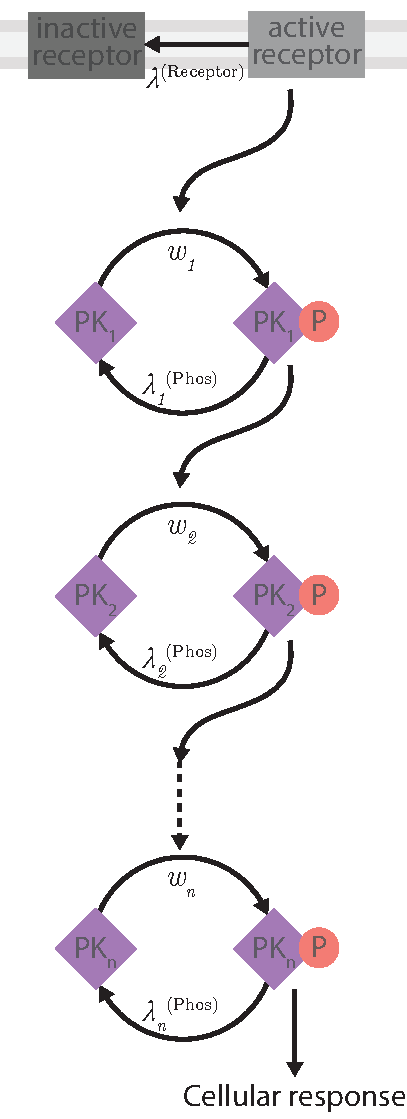
\includegraphics[width=\textwidth]{theory/fig/kinase_cascade.pdf}
\end{minipage}
\end{figure}
\end{column}
\end{columns}
\end{frame}



\section*{Questions}

